\par
\begingroup
\let\clearpage\relax
\chapter{RESULTADOS}
\label{sec:resultados}
\endgroup

São apresentados os resultados temporais e municipais dos registros classificados como dengue no Ceará entre 2016 e 2025, incluindo taxas populacionais, recorrência e distribuição espacial nos 184 municípios.

\section{Distribuição temporal dos registros}
\label{sec:resultados_temporais}

A série temporal reuniu 215.251 registros. Os maiores totais anuais ocorreram em 2016 (41.894) e 2022 (39.940), enquanto 2018 apresentou 3.995 registros, o menor valor entre 2016 e 2024. O total de 2025 requer cautela, pois sua completude não foi confirmada.

Entre março e junho, concentraram-se 141.020 registros (65,5\% do total). Maio acumulou 44.018 registros, com média anual de 4.401,8. Em todos os anos, os maiores totais mensais ocorreram entre abril e junho; o pico da série foi registrado em maio de 2022 (10.601). Essa concentração caracteriza sazonalidade descritiva, sem estabelecer associação causal com o clima.

\section{Distribuição municipal por números absolutos}
\label{sec:resultados_municipais}

A base municipal reuniu 215.243 registros válidos nos 184 municípios. Fortaleza concentrou 90.035 registros (41,83\%), seguida por Brejo Santo, com 7.249 (3,37\%), e Caucaia, com 6.155 (2,86\%). A Figura \ref{fig:top10_municipios} apresenta os dez maiores totais acumulados; essas contagens não consideram diferenças populacionais.

\begin{figure}[!htbp]
    \centering
    \captionsetup{width=16cm}
    \Caption{\label{fig:top10_municipios} Dez municípios com maiores totais acumulados de registros classificados de dengue no Ceará, 2016--2025}
    \IFCEfig{}{
        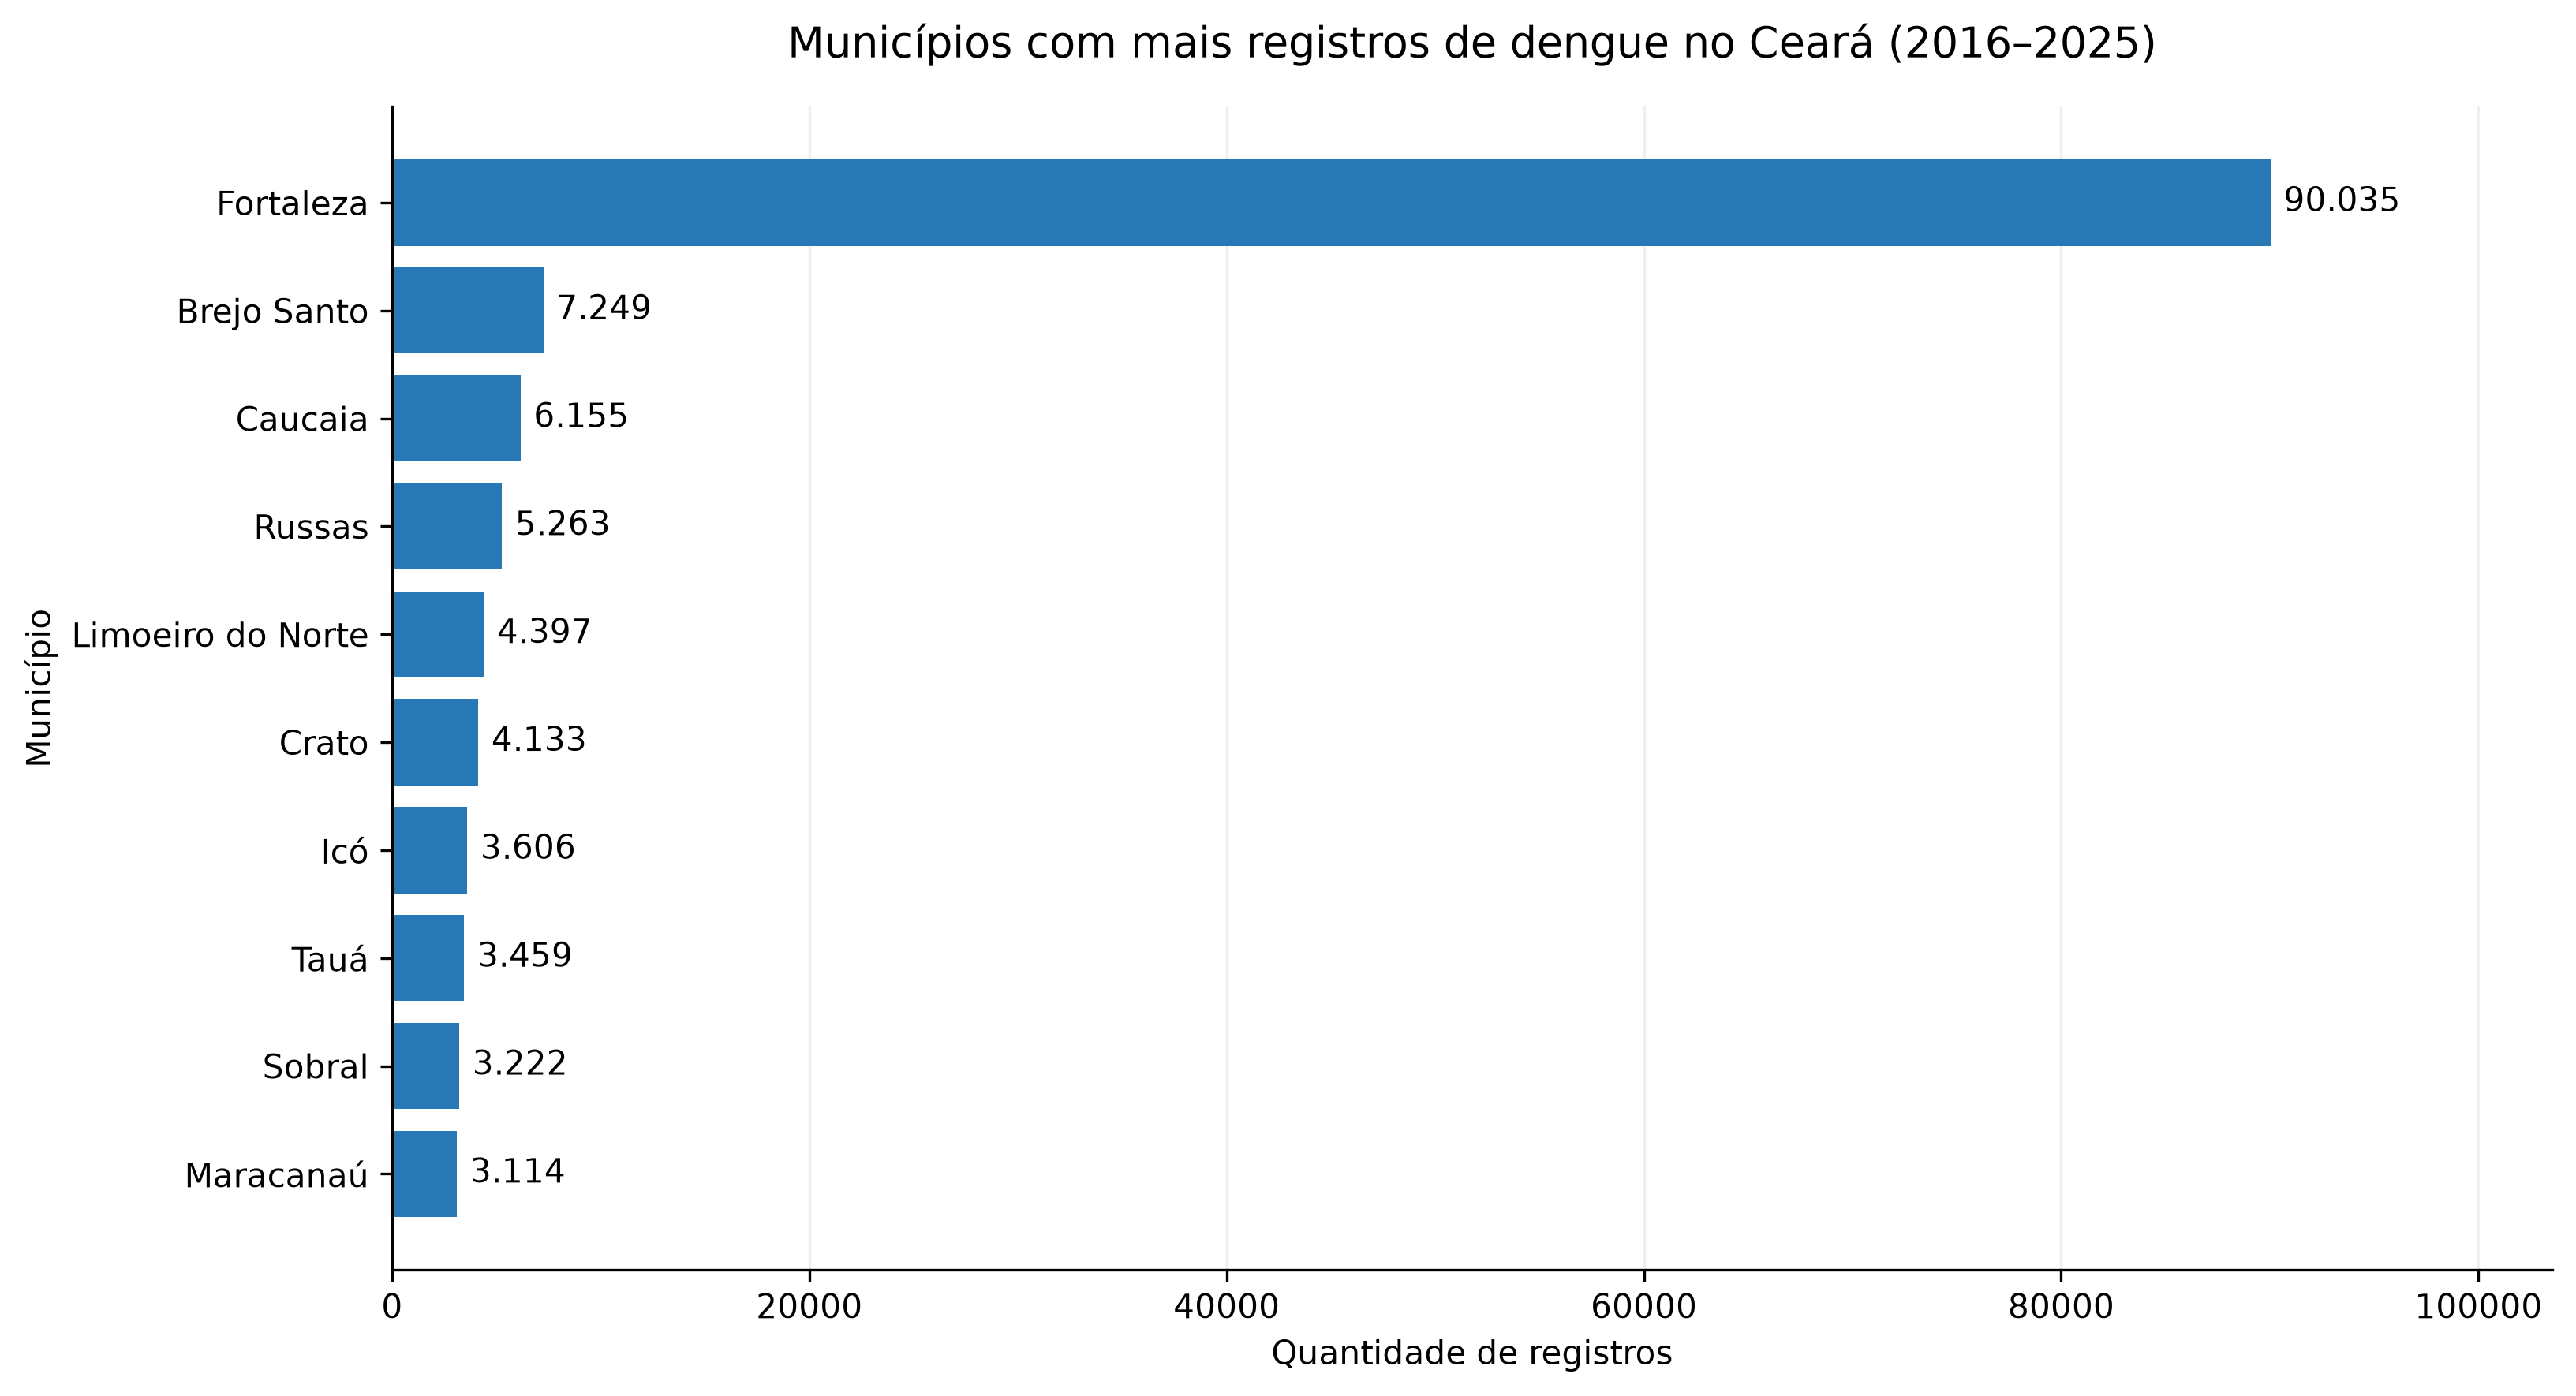
\includegraphics[width=\textwidth]{Figuras/top10_municipios_2016_2025.png}
    }{
        \Fonte{Elaborado pelo autor a partir de dados do Ministério da Saúde.}
    }
\end{figure}
\FloatBarrier

\section{Taxas anuais agregadas do Ceará}
\label{sec:resultados_taxas_estaduais}

A Tabela \ref{tab:taxas_estaduais} apresenta as taxas anuais calculadas com registros de municípios válidos e respectivas populações. As maiores ocorreram em 2016 (467,38) e 2022 (454,10), contrastando com 2018 (44,02 registros por 100 mil habitantes). Trata-se de indicadores desta pesquisa, não de taxas oficiais de incidência.

\begin{table}[!htbp]
    \centering
    \caption{Registros municipais e taxas anuais por 100 mil habitantes no Ceará, 2016--2025}
    \label{tab:taxas_estaduais}
    \small
    \begin{tabular}{rrrr}
        \toprule
        Ano & Registros & População & Taxa por 100 mil \\
        \midrule
        2016 & 41.894 & 8.963.663 & 467,38 \\
        2017 & 27.055 & 9.020.460 & 299,93 \\
        2018 & 3.995 & 9.075.649 & 44,02 \\
        2019 & 15.674 & 9.132.078 & 171,64 \\
        2020 & 21.451 & 9.187.103 & 233,49 \\
        2021 & 33.841 & 9.240.580 & 366,22 \\
        2022 & 39.938 & 8.794.957 & 454,10 \\
        2023 & 14.220 & 8.794.957 & 161,68 \\
        2024 & 12.127 & 9.233.656 & 131,33 \\
        2025 & 5.048 & 9.268.836 & 54,46 \\
        \bottomrule
    \end{tabular}

    \vspace{0.2cm}
    \begin{minipage}{\textwidth}
        \footnotesize
        Fonte: elaboração própria a partir de dados do Ministério da Saúde e do IBGE.

        Nota: os totais municipais excluem oito registros sem município cearense válido. A população de 2023 utiliza referência baseada no Censo de 2022.
    \end{minipage}
\end{table}
\FloatBarrier

\section{Evolução das taxas de Brejo Santo e do Ceará}
\label{sec:brejo_ceara}

Conforme a Figura \ref{fig:brejo_ceara}, Brejo Santo superou a taxa estadual em oito dos dez anos, exceto em 2016 e 2021. Suas taxas em 2017, 2023 e 2024 foram, respectivamente, de 2.877,33, 3.491,88 e 4.425,60 registros por 100 mil habitantes, equivalentes a cerca de 9,59, 21,60 e 33,70 vezes as taxas estaduais. A comparação não identifica as causas dessas diferenças.

\begin{figure}[!htbp]
    \centering
    \captionsetup{width=12cm}
    \Caption{\label{fig:brejo_ceara} Evolução das taxas de registros classificados de dengue em Brejo Santo e no Ceará, 2016--2025}
    \IFCEfig{}{
        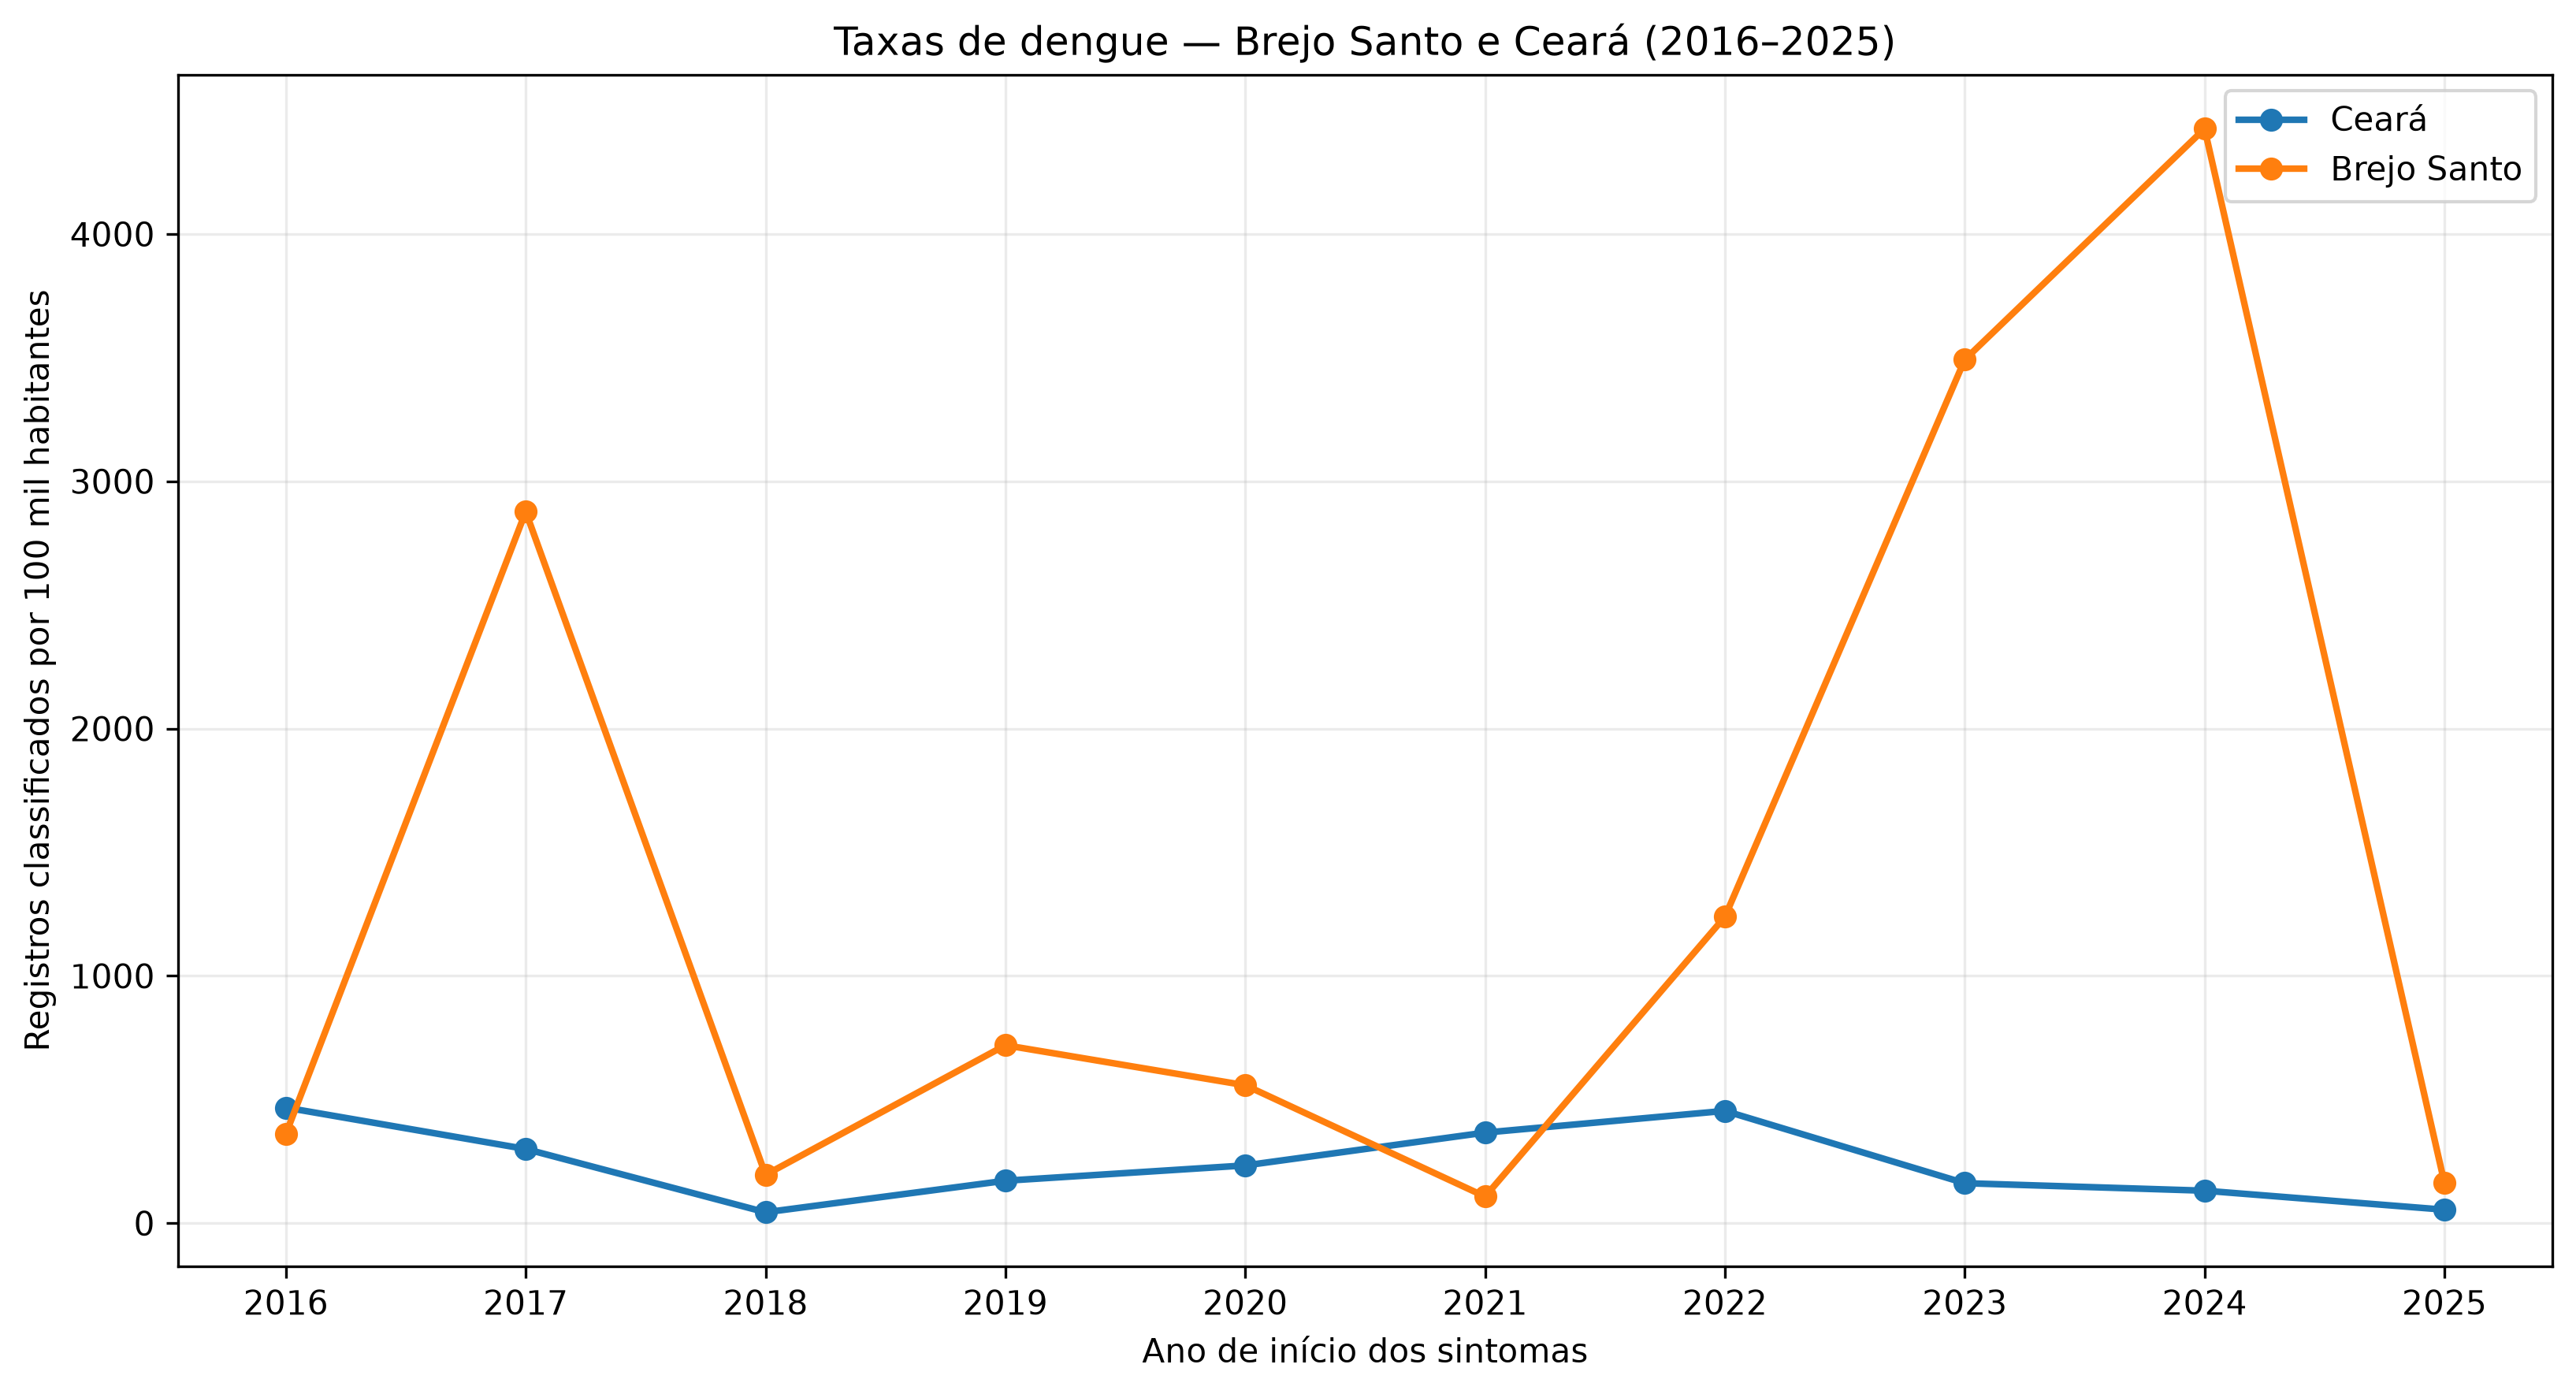
\includegraphics[width=\textwidth,height=\textheight,keepaspectratio]{Figuras/comparativo_brejo_ceara_2016_2025.png}
    }{
        \Fonte{Elaborado pelo autor a partir de dados do Ministério da Saúde e do IBGE.}
    }
\end{figure}
\FloatBarrier

\section{Recorrência de taxas municipais superiores à estadual}
\label{sec:recorrencia_municipal}

Brejo Santo, Quixeré, Tabuleiro do Norte e Fortaleza apresentaram taxas superiores à estadual em oito dos dez anos; Penaforte, Icapuí, Jaguaribara e Limoeiro do Norte, em sete. A Figura \ref{fig:heatmap_municipal} compara as taxas anuais dos 15 municípios selecionados por maior recorrência, evidenciando variações entre municípios e anos. A recorrência expressa posição relativa à taxa estadual, não taxas necessariamente elevadas em termos absolutos.

\begin{figure}[!htbp]
    \centering
    \captionsetup{width=16cm}
    \Caption{\label{fig:heatmap_municipal} Taxas anuais dos 15 municípios selecionados por maior recorrência acima da taxa estadual, 2016--2025}
    \IFCEfig{}{
        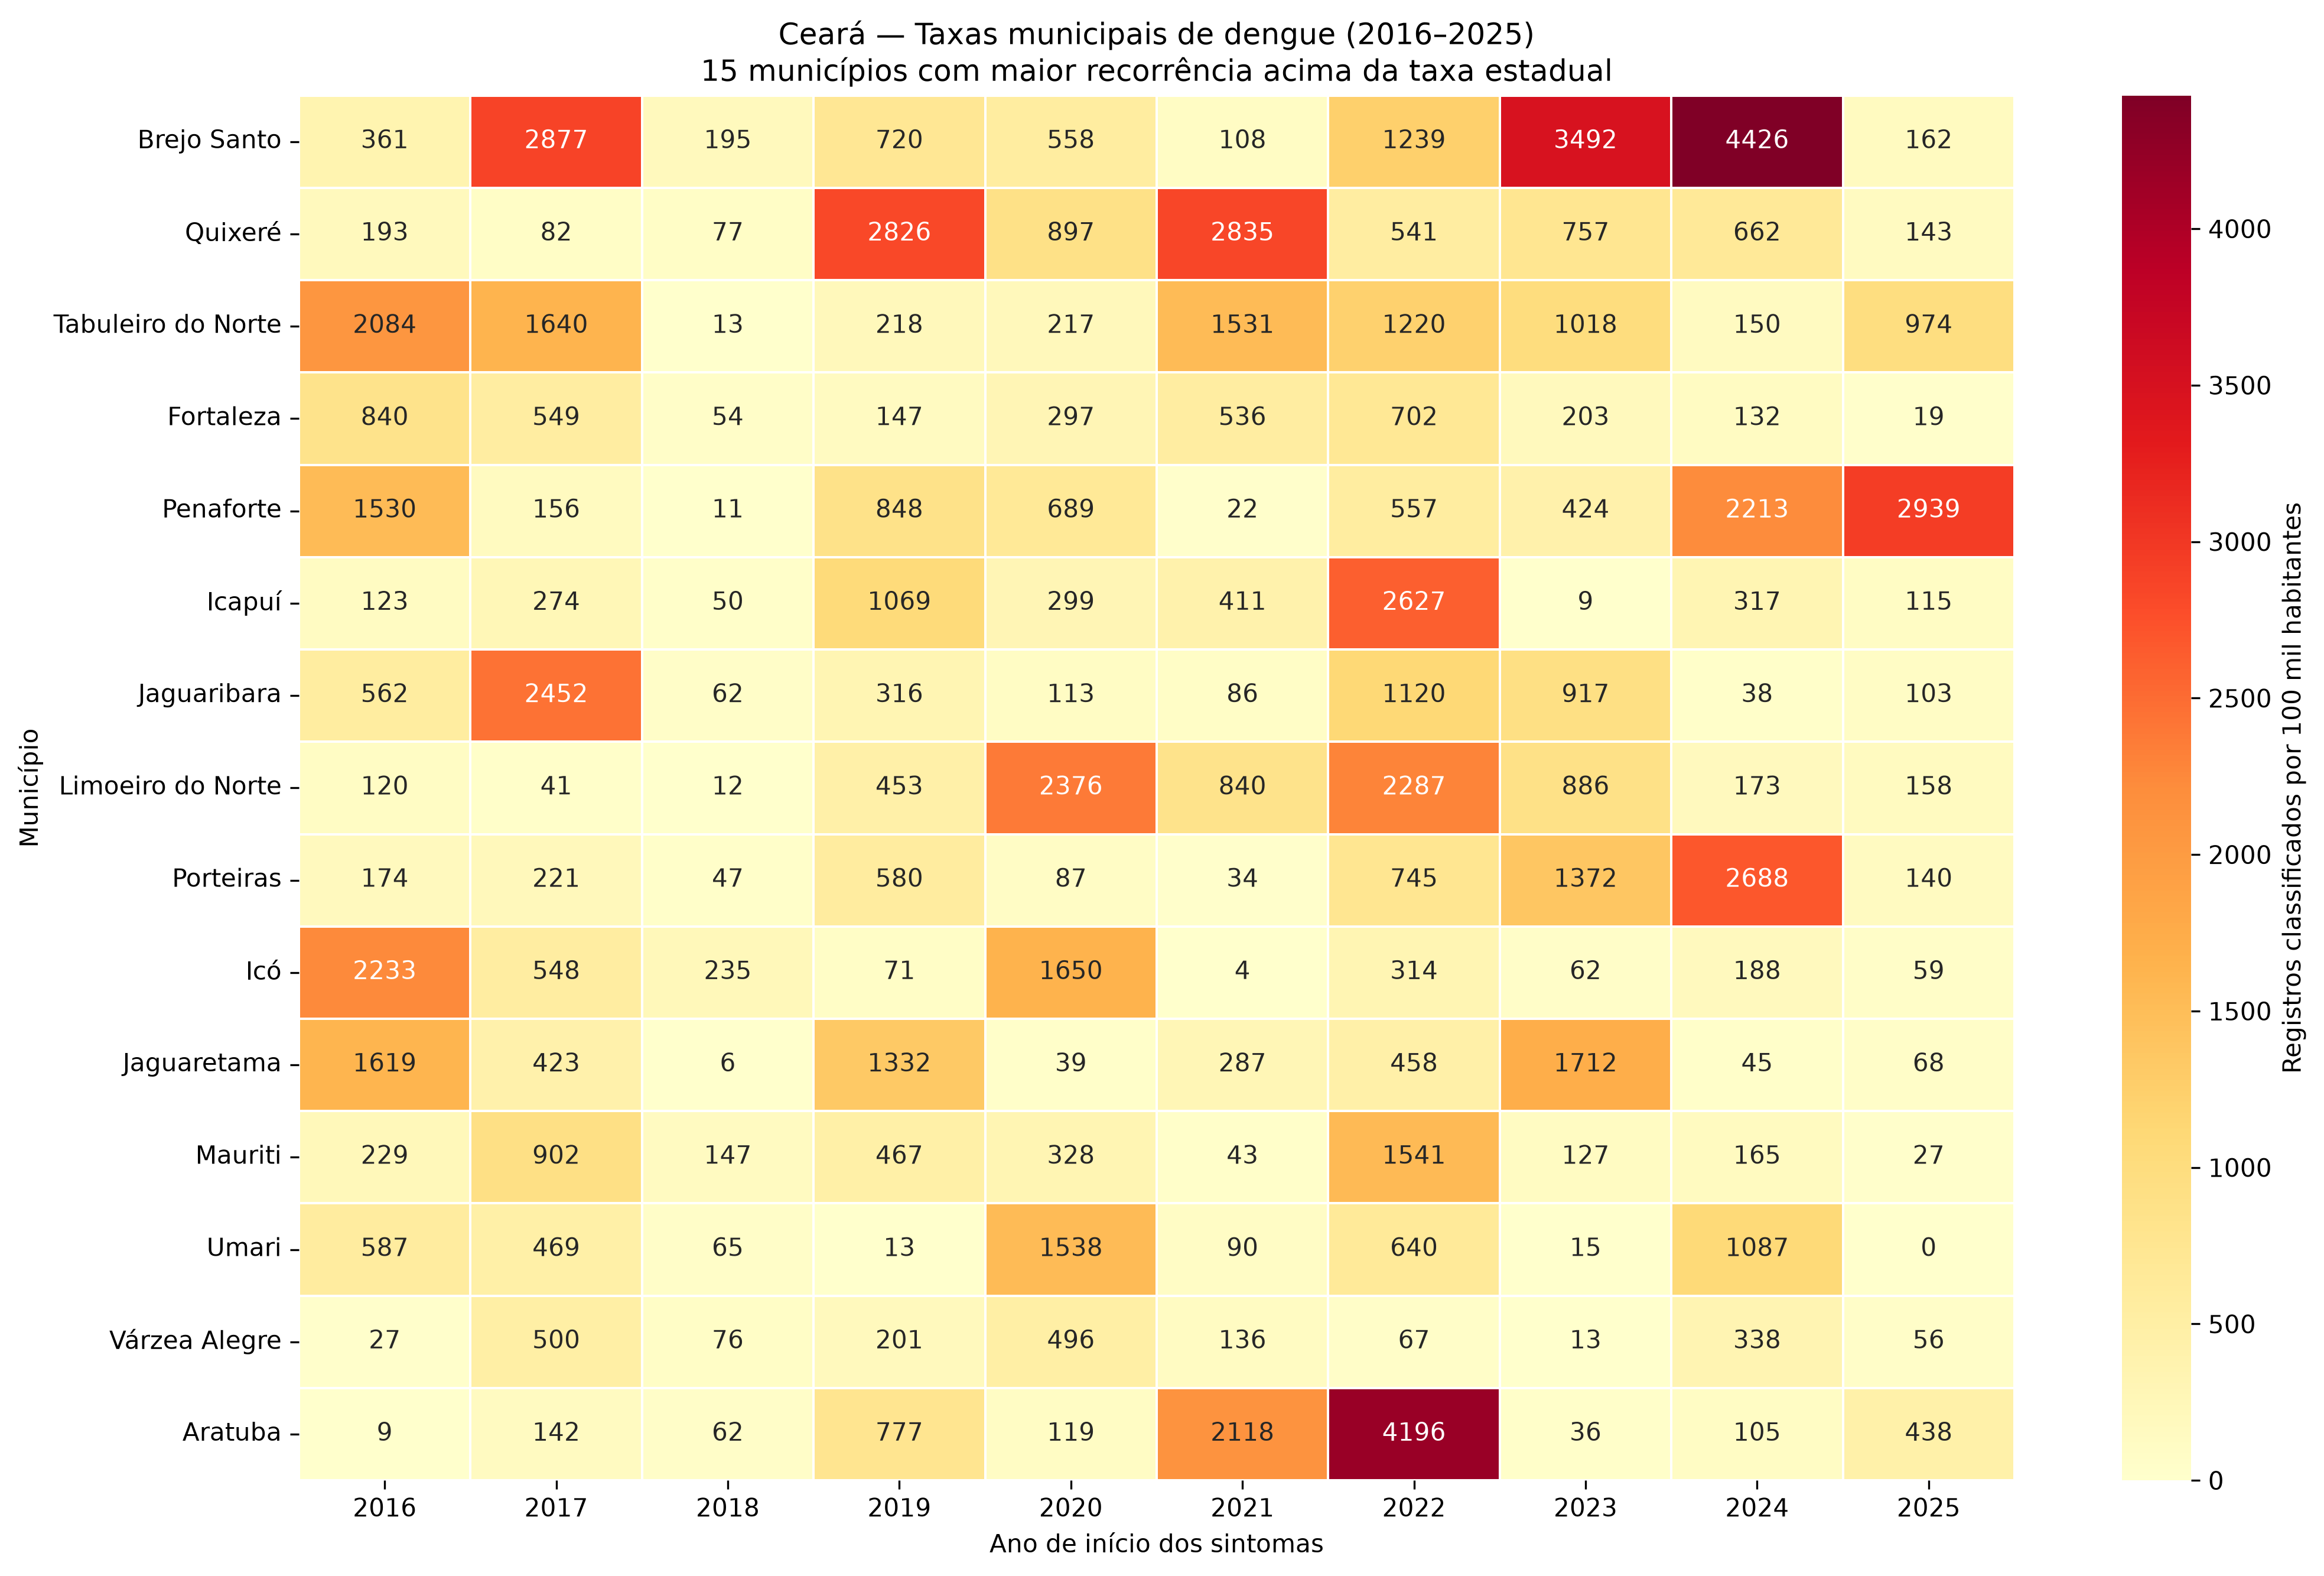
\includegraphics[width=\textwidth]{Figuras/heatmap_taxas_municipais.png}
    }{
        \Fonte{Elaborado pelo autor a partir de dados do Ministério da Saúde e do IBGE.}
    }
\end{figure}
\FloatBarrier

\section{Distribuição espacial das taxas municipais}
\label{sec:resultados_espaciais}

Os mapas históricos (Figura \ref{fig:mapas_historicos}) mostram variação espacial das taxas nos 184 municípios. O número de municípios com taxas superiores a 700 registros por 100 mil habitantes foi de 27 em 2022, dois em 2018, 22 em 2016 e em 2021 e nove em 2024. Em 2016, 11 municípios superaram 1.500 registros por 100 mil habitantes, o maior total nessa faixa na série.

As classes dos mapas são descritivas e constantes durante a série, permitindo comparação visual sem comprovar agrupamentos espaciais estatisticamente significativos.

\begin{figure}[!htbp]
    \centering
    \captionsetup{width=16cm}
    \Caption{\label{fig:mapas_historicos} Distribuição municipal das taxas de registros classificados de dengue no Ceará, 2016--2025}
    \IFCEfig{}{
        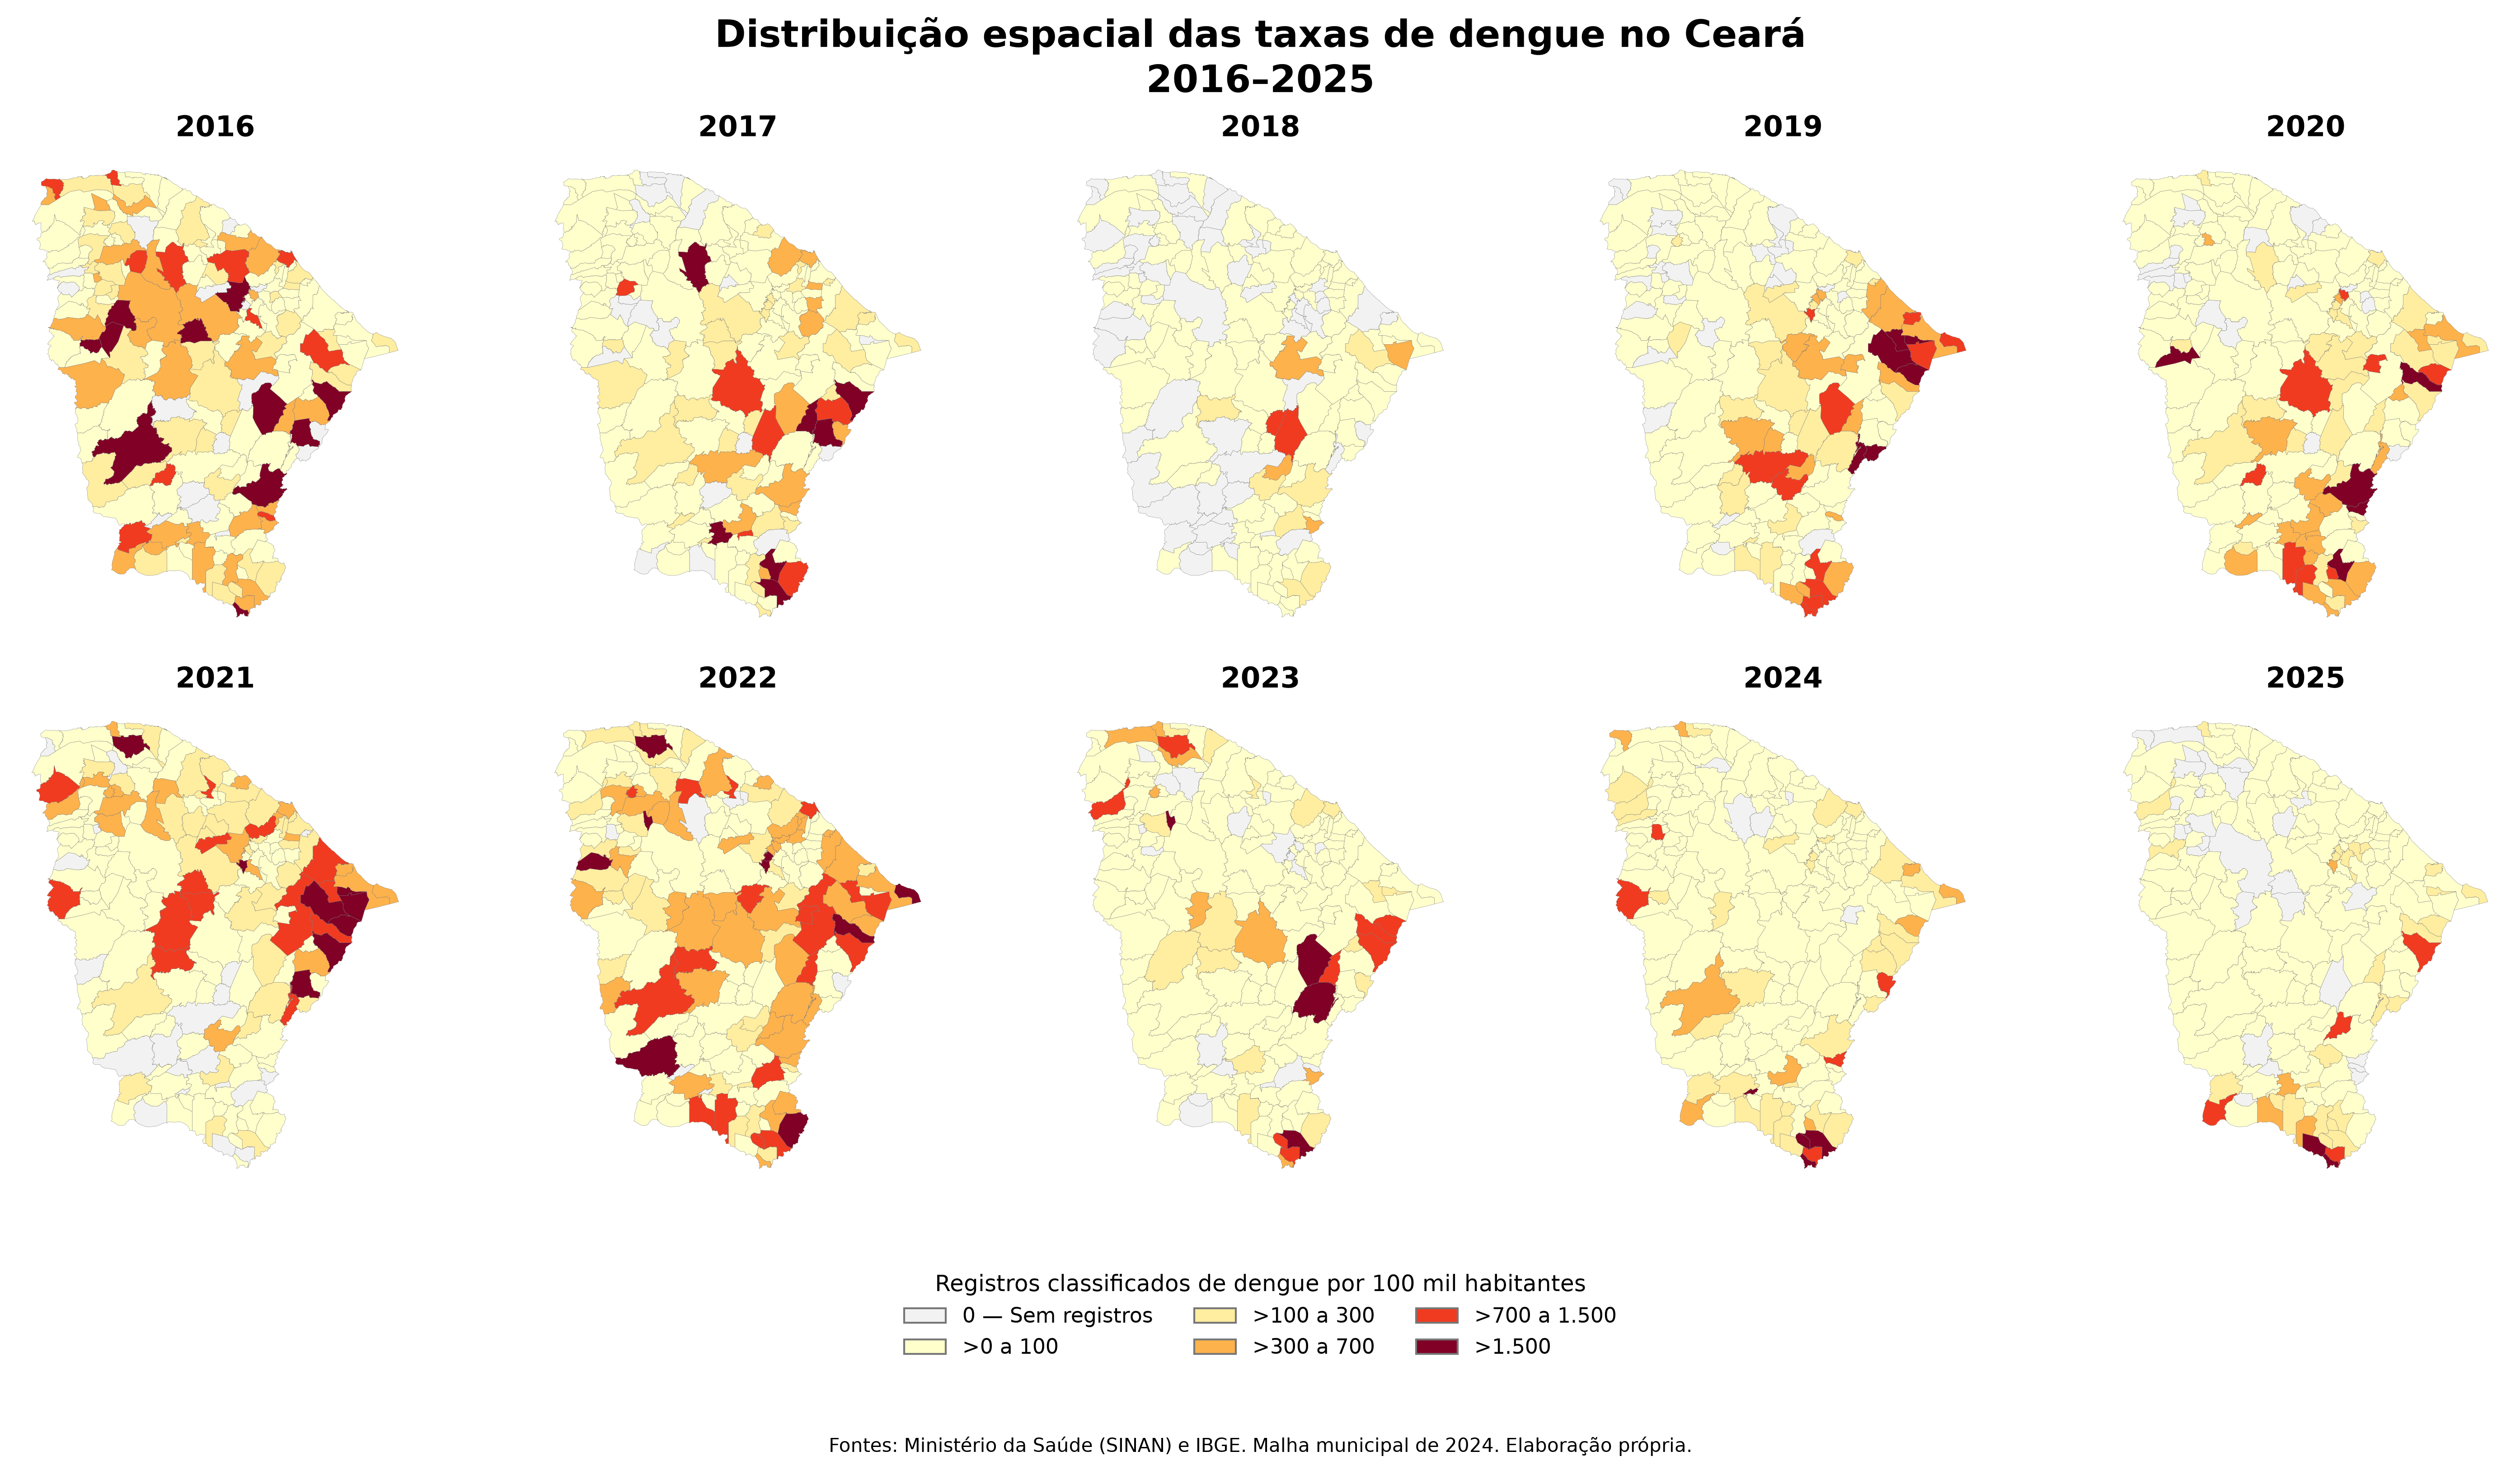
\includegraphics[width=\textwidth]{Figuras/mapas_historicos_dengue_2016_2025.png}
    }{
        \Fonte{Elaborado pelo autor a partir de dados do Ministério da Saúde e do IBGE.}
    }
\end{figure}
\FloatBarrier

\section{Limitações na interpretação dos resultados}
\label{sec:limitacoes_resultados}

A interpretação depende da qualidade das classificações, de possíveis duplicidades e das fontes populacionais. A exclusão dos 62 registros com intervalo superior a 365 dias pode afetar as agregações; a referência populacional de 2023 baseia-se no Censo de 2022 e a completude de 2025 não foi confirmada. A malha municipal de 2024 foi aplicada aos dez anos. Assim, contagens e taxas não equivalem necessariamente a casos únicos ou à incidência oficial, e os padrões observados não demonstram causalidade nem dependência espacial significativa.
